\section{Image Reconstruction for MeerKAT} \label{intro}
In the real world, measurements are corrupted by noise. Noise is introduced by the measurement instrument itself, but additional interference sources may be present. For example in Audio Recording, the microphone measures a noisy signal from the real world tone, and a passing car introduces additional interference. In a controlled environment like a recording studio, sound proofing handles the interference and only the noisy measurements have to be dealt with. Controlled environments are not always possible, that's why in Signal Processing the fields of de-noising and reconstruction exists. With those, we want to reconstruct the truly observed signal without the noise or external interference.

Image de-noising and reconstruction problems appear in different fields. In Astronomy, Radio Interferometers pose a challenging image reconstruction problem. The Interferometer measures a noisy image of the sky, corrupted by various sources like the ionosphere, passing satellites and the Interferometer itself. In the past, reconstruction algorithms used simple approximations to correct the image. For new interferometers like MeerKAT the approximations of the past do not hold. Furthermore, the larger MeerKAT instrument poses the reconstruction problem on a new data volume.

CLEAN algorithm\cite{rich2008multi}\cite{rau2011multi}

Reconstruction algorithms for MeerKAT should handle the more complex effects of ionosphere and the like, while scaling even more on larger problem instances. Reconstruction algorithms using the theory of compressed sensing\cite{candes2006robust}\cite{donoho2006compressed} showed higher reconstruction accuracy than state of the art algorithms. However, they currently do require more computing hardware. This project searches for a way to make CS Algorithm scale on MeerKAT data size.

SASIR\cite{starck2015starlet} or more recently reconstructions using SARA \cite{dabbech2018cygnus} \cite{birdi2018sparse}

super resolution

\subsection{The basic Measurement Equation of a radio interferometer}\label{intro:basic}
Real world radio interferometers have complicated measurement equations. They become even more complicated for large interferometers like MeerKAT. These problems get addressed in section \ref{meerkat}. This section looks at the basic measurement equation of a radio interferometer \eqref{intro:measurement} and discusses the two fundamental challenges for image reconstruction. 

\begin{equation}\label{intro:measurement}
V(u, v) = \int\int I(x, y) e^{2 \pi i (ux+vy)} \: dx \: dy
\end{equation}

An interferometer measures Fourier Components $V$ (called Visibilities in Radio Astronomy) from the sky image $I$ at position $x$ and $y$. The term $e^{2 \pi i (ux+vy)}$ represents the two dimensional Fourier Transform. The task is to reconstruct the observed image $I$ from the measured Visibilities $V$. In theory this task is trivial: Since the inverse Fourier Transform exists, we can reconstruct the image $I$ by calculating the inverse Fourier Transform of $V$. However, two properties of the Visibilities make this task challenging in practice:

\begin{enumerate}
	\item Non-uniform sampling pattern in Visibility space
	\item Incomplete Visibility coverage. 
\end{enumerate} 

\textit{Property 1:} We want to reconstruct an image with uniformly spaced pixels. The instrument defines the sampling pattern in Visibility space and does not correspond to the exact pixels of the reconstructed image. This property keeps us from using the Fast Fourier Transform. The naive inverse Fourier Transform can still be calculated, but it has a quadratic runtime and does not scale to the data volume of interferometers. Current reconstruction algorithms use the non-uniform Fast Fourier Transform (nuFFT). The nuFFT approximates the non-uniform Fourier Transform. 

\textit{Property 2:} Interferometers sample only a limited set of Visibilities. It does not have the whole information for reconstruction. This has the effect that the instrument introduces fake structures into the image. With only knowing the incomplete set of Visibilities, a reconstruction algorithm has to decide which image structures were truly measured, and which are due to the instrument. This forms an ill-posed inverse problem. There are many images that fit the measurements, and a small change in the Visibilities can lead to a very different reconstruction. 

The CLEAN algorithms approximate the observed image with a deconvolution: The inverse Fourier Transform produces a corrupted image. The observed image was convolved with a known Point Spread Function (PSF), which represents the instrument. Finding a deconvolution reconstructs the observed image. The deconvolution is still an ill-posed problem, there are potentially many possible deconvolutions, and a small change in the input can lead to a very different output. Furthermore the CLEAN algorithms produce a greedy approximation of the deconvolution. 

A CLEAN image reconstruction uses two different approximation algorithms: The nuFFT, which approximates the inverse Fourier Transform, and the CLEAN deconvolution, which approximately removes instrumental effects. In real world reconstructions, these two approximations are used in the major cycle architecture to further increase its accuracies.

\subsection{The Major Cycle Architecture}
Major cycle was created with CLEAN in mind, but the CS approaches use a similar architecture

An image reconstruction for radio interferometers consists of two different steps: A nuFFT, which approximates the inverse Fourier Transform efficiently and an image constraint/deconvolution algorithm, which approximates the instrumental effects on the image (for example CLEAN). These two approximations are an error source of the reconstruction. The major cycle architecture \ref{intro:major} therefore tries to iteratively minimize the errors of the nuFFT and the deconvolution.

\begin{wrapfigure}{r}{0.6\textwidth}
	\centering
	\vspace{-10pt}
	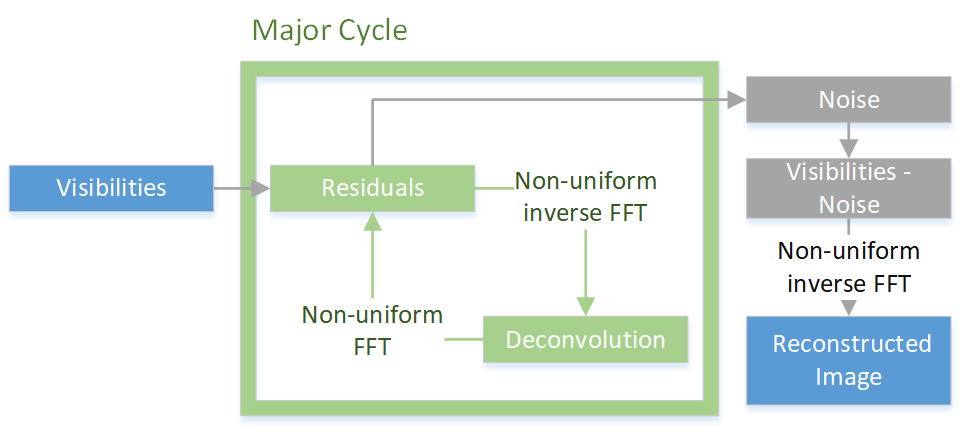
\includegraphics[width=1.0\linewidth]{./chapters/01.intro/Major-Minor.png}
	\caption{The Major Cycle Framework}
	\label{intro:major}
	\vspace{-10pt}
\end{wrapfigure}

The first major cycle uses the non-uniform inverse FFT to approximate the 'dirty' image from the Visibilities. The image constraint/Deconvolution algorithm decides parts which parts belong to the observed image and which are due to instrumental effects and other noise sources. It then returns the noise part, which get transformed back into residual Visibilities. The next major cycle iteration continues with the residual Visibilities. The residual Visibilities get minimized until they contain only the instrumental effects and noise.

After several major cycles the residual  on a regularly spaced image which has a small error from non-uniform samples, and a small error from incomplete measurements.

A single major cycle is expensive. MeerKAT needs several cycles to have a good image result with a CLEAN algorithm.


Compressed Sensing as a deconvolution.

Slightly different implementation in Compressed Sensing approaches, does not neatly fit in the figure \ref{intro:major}, but still gains the same advantages and disadvantages as the standard major cycle. 

Compressed Sensing algorithms use essentially the same architecture. But in turn uses more major cylces, on top of being more expensive to compute inside a cycle. Even though it was shown to produce better reconstructions on different datasets, the added runtime is a big reason what keeps it from wide-spread adoption. 

The question thefore is, can the overall complexity of the comporessed sensing reconstruction be reduced, if a different architecture is used.


\subsection{Compressed Sensing Reconstructions}
 However, compressed Sensing algorithms come with the drawback of requiring more major cycles.

MeerKAT due to wide field of view introduces even more troubles

Current Compressed Sensing reconstructions reduce the number of major cycles. However, the question is if Compressed Sensing can use a different architecture, and scale better to problems of the size of MeerKAT.

Furthermore on the new MeerKAT instruments, we have a big data problem. We want to create a large image from a large amount of Visibilities. 32k*32k pixels and terabytes of raw Visibility data. 

Scalability is a big problem.

There are ways to get rid of the major cycle, but overall the complexity could not be reduced.









